\chapter{Work sharing}

\section{Unmodified program}

\begin{figure}[!h]
  \begin{center}
         \resizebox{160mm}{!}{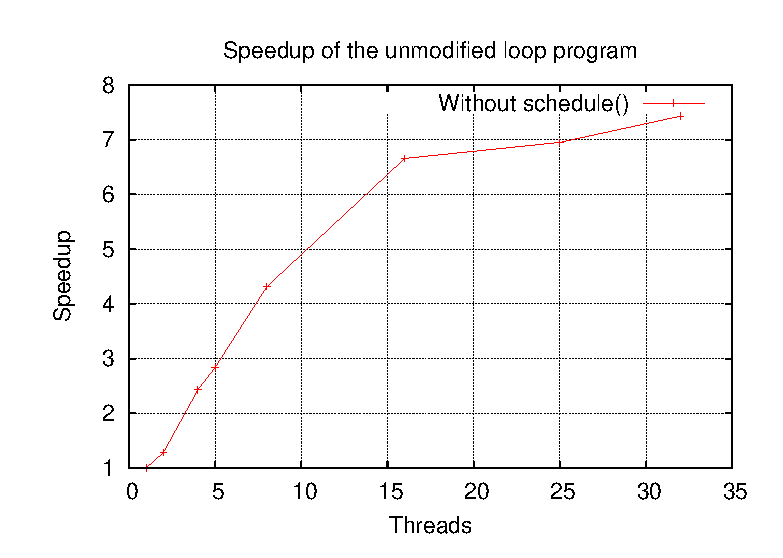
\includegraphics{pic/graph_q4.eps}}
  \end{center}
  \caption{Speedup of the unmodified program}
  \label{unmodif}
\end{figure}

\section{Using scheduling directives}

In the graphs \ref{2000} and \ref{10000}, we tried the three directives with an arbitrary sized chunk. The graph \ref{opt} shows the result if we let OpenMP take care of the chunk's size.

\begin{figure}[!h]
  \begin{center}
         \resizebox{160mm}{!}{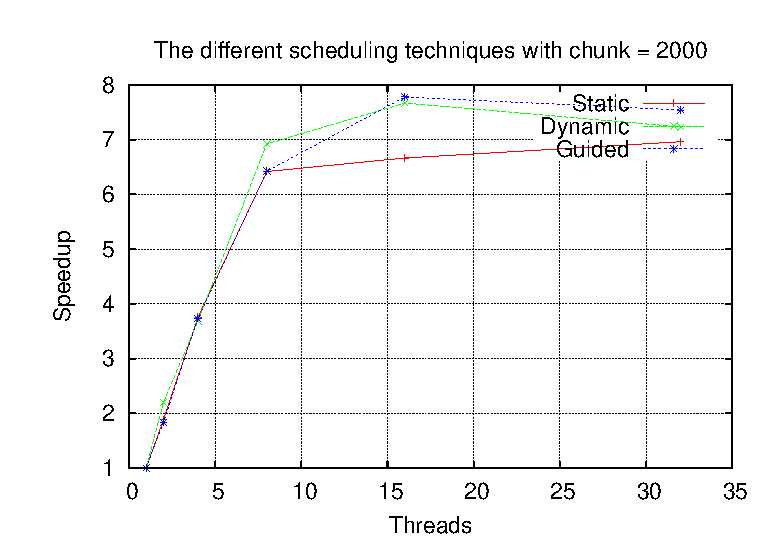
\includegraphics{pic/graph_q4_2000.eps}}
  \end{center}
  \caption{With chunk = 2000}
  \label{2000}
\end{figure}

\begin{figure}[!h]
  \begin{center}
         \resizebox{160mm}{!}{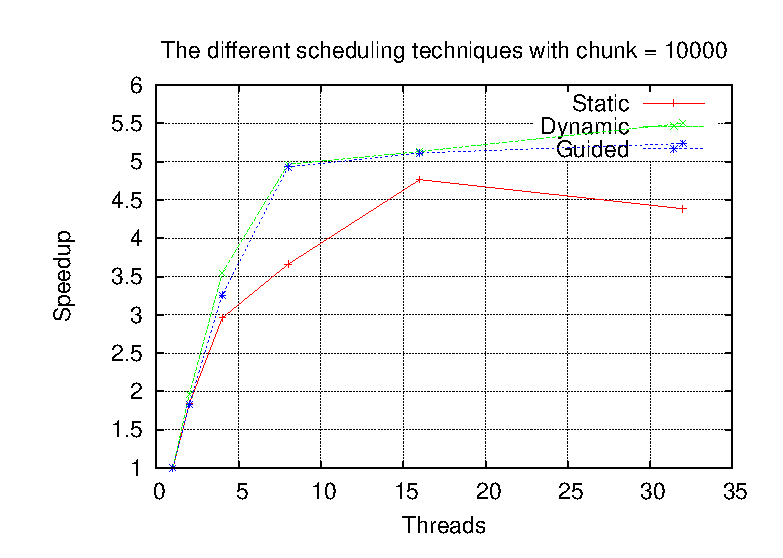
\includegraphics{pic/graph_q4_10000.eps}}
  \end{center}
  \caption{With chunk = 10000}
  \label{10000}
\end{figure}

\begin{figure}[!h]
  \begin{center}
         \resizebox{160mm}{!}{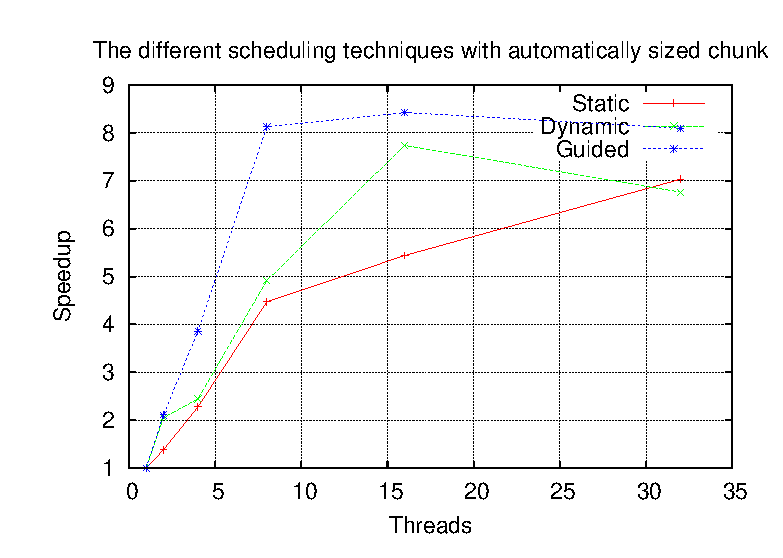
\includegraphics{pic/graph_q4_opt.eps}}
  \end{center}
  \caption{With automatically sized chunk}
  \label{opt}
\end{figure}

As we can see, choosing dynamic or guided scheduling gives the bests results. It is so because the problem was a poor load balance and it is known that both dynamic and guided scheduling are good to avoid this problem.
